\section{Model Architecture}
\label{sec:model_architecture}

\chonk is a Transformer-based encoder model that resembles the architecture of the original Vision Transformer~\citep{dosovitskiy2020image} but incorporates the following three main modifications to improve efficiency and training stability at scale: parallel layers, query/key (QK) normalization, and omitted biases.


\paragraph{Parallel layers.}
As in \citet{gpt-j}, \chonk applies the Attention and MLP blocks in parallel, instead of sequentially as in the standard Transformer:
 \begin{align*} 
 y' &= \text{LayerNorm}(x),\\
 y\hphantom{'} &= x + \text{MLP}(y')+\text{Attention}(y').
 \end{align*}
%  where ``LN()'' stands for the Layer Normalization (LayerNorm)~\citep{ba2016layer} function,
This enables additional parallelization via combination of linear projections from the MLP and attention blocks. In particular, the matrix multiplication for query/key/value-projections and the first linear layer of the MLP are fused into a single operation, and the same is done for the attention out-projection and second linear layer of the MLP. This approach is also used by PaLM~\citep{chowdhery2022palm}, where this technique sped up the largest model's training by 15\% without performance degradation. 
    
\paragraph{QK Normalization.}
In scaling ViT beyond prior works, we observed divergent training loss after a few thousand steps. In particular, this instability was observed for models with around 8B parameters (see \cref{app:scalability}). It was caused by extremely large values in attention logits, which lead to (almost one-hot) attention weights with near-zero entropy.
To solve this, we adopt the approach of \citet{gilmer2023intriguing}, which applies LayerNorm~\citep{ba2016layer} to the queries and keys before the dot-product attention computation.
Specifically, the attention weights are computed as
\begin{align*}
%\text{softmax}\left[ \frac{\text{LN}(X W^Q) ( \text{LN}(X W^K))^T}{\sqrt{d}}\right],
% moved the big division by sqrt-d into a small factor at the front, feel free to revert; could also be d^{-1/2} of course.
\text{softmax}\left[  \tfrac{1}{\sqrt{d}}
{\text{LN}(X W^Q) ( \text{LN}(X W^K))^T} \right],
\end{align*}
where $d$ is query/key dimension, $X$ is the input, $\text{LN}$ stands for layer normalization, and $W^Q$ is the query weight matrix, and $W^K$ is the key weight matrix.
The effect on an 8B parameter model is shown in \cref{fig:stability_8b}, where normalization prevents divergence due to uncontrolled attention logit growth.
%
\begin{figure}[tbp]
    \centering
    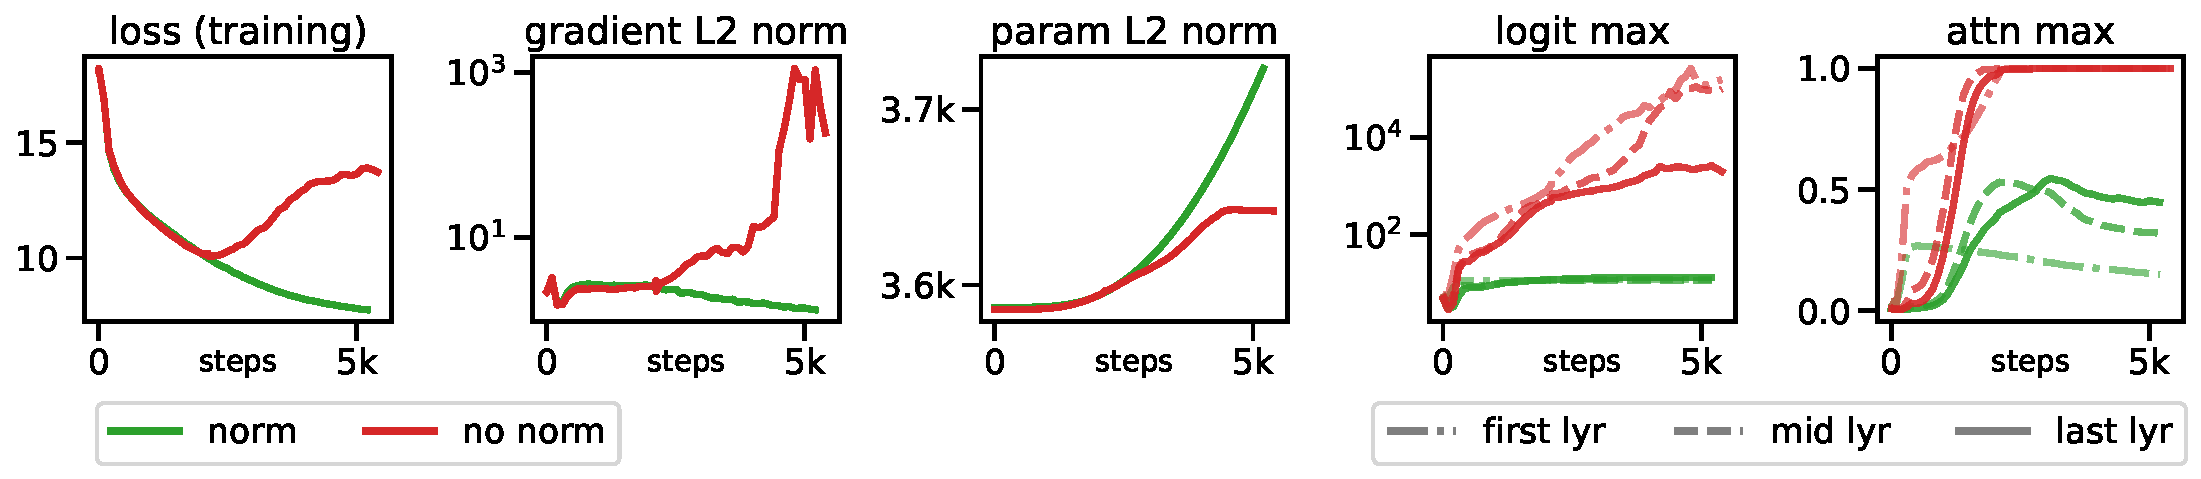
\includegraphics[width=\textwidth]{figs/stability_8b_1line.pdf}
    % \vspace{-10pt}
    \caption{Effect of query/key normalization on an 8B parameter model.}
    % \vspace{-16pt}
    \label{fig:stability_8b}
\end{figure}
% In addition, we re-scale the query after the normalization with $\sfrac{1}{\sqrt{d}}$, where $d$ is the query dimension. 
%The model parallelism on the attention layer of \chonk is done by partitioning the computation on the ``head" axis. Thus to avoid the need for a synchronous all-reduce needed for query/key LayerNorms, we used statistics from a group of heads instead of all of them, which reduced the communication without affecting performance. 
    
\paragraph{Omitting biases on QKV projections and LayerNorms.}
Following PaLM~\citep{chowdhery2022palm}, the bias terms were removed from the QKV projections and all LayerNorms were applied without bias and centering~\citep{zhang2019root}. This improved accelerator utilization (by 3\%), without quality degradation. However, unlike PaLM, we use bias terms for the (in- and out-) MLP dense layers as we have observed improved quality and no speed reduction. 

\begin{figure}[t]
    % \vspace{-5pt}
    \centering
    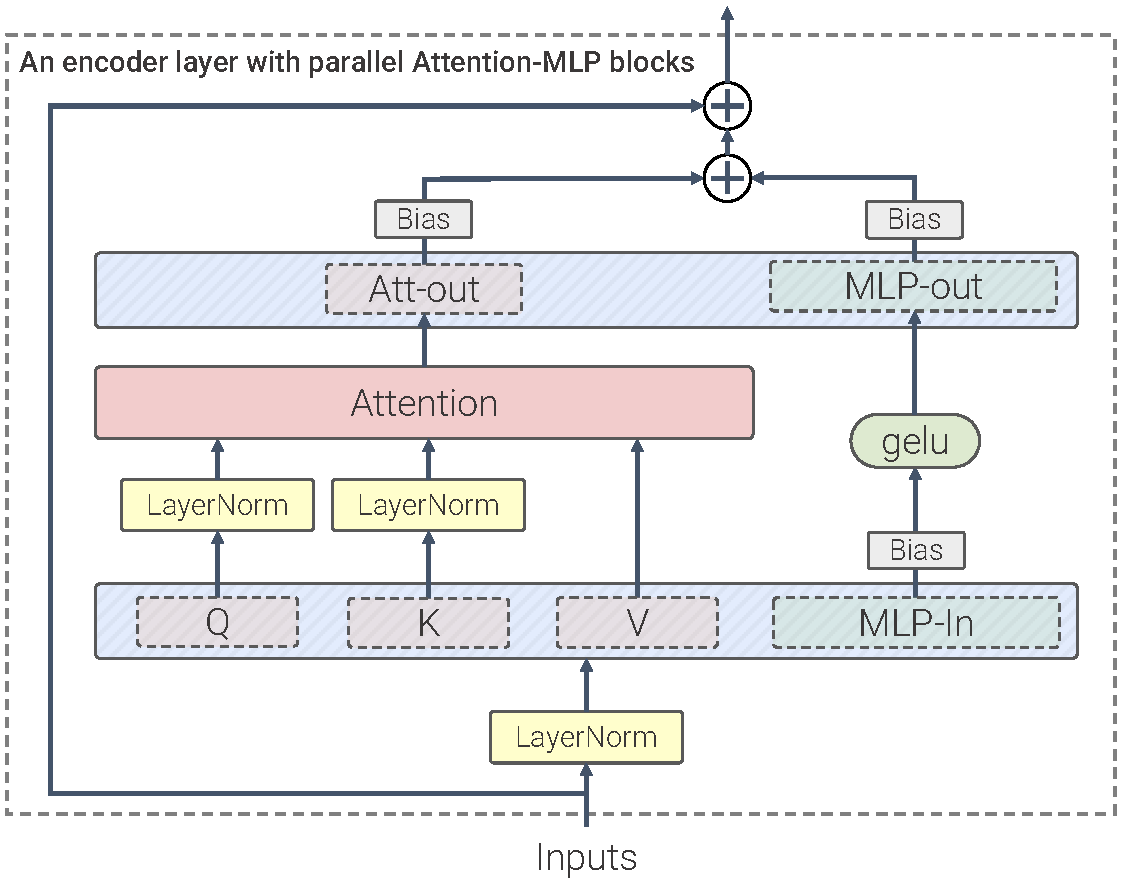
\includegraphics[width=0.6\textwidth]{figs/vit22b_new.pdf}
    % \vspace{-10pt}
    \caption{Parallel \chonk layer with QK normalization.}
    \label{fig:vit22b_schema}
    % \vspace{-15pt}
\end{figure}

\cref{fig:vit22b_schema} illustrates a \chonk encoder block. The embedding layer, which includes extracting patches, linear projection, and the addition of position embedding follow those used in the original ViT. We use multi-head attention pooling~\citep{cordonnier2019relationship,zhai2022scaling} to aggregate the per-token representations in the head. 

\chonk is uses patch size of $14 \times 14$ with  images at resolution $224 \times 224$ (pre-processed by inception crop followed by random horizontal flip). 
Similar to the original ViT~\citep{dosovitskiy2020image}, \chonk employs a learned 1D positional embedding. 
During fine-tuning on high-resolution images (different number of visual tokens), we perform a 2D interpolation of the pre-trained position embeddings, according to their location in the original image. 

Other hyperparameters for the \chonk model architecture are presented in \cref{tbl:model_arch}, compared to the previously reported largest ViT models, ViT-G~\citep{zhai2022scaling} and ViT-e~\citep{chen2022pali}.

\begin{table}[h]
  \caption{\chonk model architecture details.}
  \centering
  \begin{tabulary}{1.0\linewidth}{@{}LCCCCR@{}}
    \toprule
    \bf{Name} & \bf{Width} & \bf{Depth} & \bf{MLP} & \bf{Heads} & \bf{Params [M]} \\
           %G/14
          ViT-G & 1664 & 48 & \phantom{0}8192  & 16 & 1843  \\
           %e/14  
          ViT-e & 1792 & 56 & 15360 & 16 & 3926  \\
    \textbf{\chonk} & 6144 & 48 & 24576 & 48 & 21743 \\
    \bottomrule
  \end{tabulary}
  \label{tbl:model_arch}
\end{table}


Following the template in~\citet{mitchell2019model}, we provide the model card in \Cref{tab:model_card} (\Cref{app:model_card}).
%\todo{Mostafa: Complete the model card.}